\documentclass{article}
\usepackage{booktabs}
\usepackage{caption}
\usepackage{subcaption}
\usepackage{float}
\usepackage{geometry}
\usepackage{pdflscape}
\geometry{margin=1in}

\begin{document}

\title{Analysis Results}
\author{Your Name}
\date{}

\maketitle

\section{Municipality Level Specification}
\subsection{First stage}
\begin{table}[htbp]\centering
\def\sym#1{\ifmmode^{#1}\else\(^{#1}\)\fi}
\caption{Raw Splits}
\begin{tabular}{l*{3}{c}}
\hline\hline
                    &\multicolumn{1}{c}{(1)}&\multicolumn{1}{c}{(2)}&\multicolumn{1}{c}{(3)}\\
                    &\multicolumn{1}{c}{Municipality Touches Principle City}&\multicolumn{1}{c}{Length to center city (edge-edge)}&\multicolumn{1}{c}{above\_len\_med}\\
\hline
Incorporated 1940-70&       0.143\sym{***}&   -6162.352\sym{***}&      -0.156\sym{***}\\
                    &     (0.017)         &  (1542.008)         &     (0.029)         \\
[1em]
Above Median GM     &       0.017\sym{**} &   -3854.789\sym{***}&      -0.056\sym{***}\\
                    &     (0.007)         &   (661.713)         &     (0.012)         \\
[1em]
Above Median GM X Inc. 1940-70&      -0.030         &   -6751.830\sym{***}&      -0.112\sym{***}\\
                    &     (0.021)         &  (1899.496)         &     (0.036)         \\
[1em]
Constant            &       0.065\sym{***}&   34591.827\sym{***}&       0.573\sym{***}\\
                    &     (0.006)         &   (529.099)         &     (0.010)         \\
\hline
Observations        &        7728         &        7595         &        7728         \\
\(R^{2}\)           &       0.021         &       0.027         &       0.029         \\
\hline\hline
\multicolumn{4}{l}{\footnotesize Standard errors in parentheses}\\
\multicolumn{4}{l}{\footnotesize \sym{*} \(p<0.10\), \sym{**} \(p<0.05\), \sym{***} \(p<0.01\)}\\
\end{tabular}
\end{table}

\begin{table}[htbp]\centering
\def\sym#1{\ifmmode^{#1}\else\(^{#1}\)\fi}
\caption{0-th Stage}
\begin{tabular}{l*{3}{c}}
\hline\hline
                    &\multicolumn{1}{c}{(1)}&\multicolumn{1}{c}{(2)}&\multicolumn{1}{c}{(3)}\\
                    &\multicolumn{1}{c}{Municipality Touches Principle City}&\multicolumn{1}{c}{Length to center city (edge-edge)}&\multicolumn{1}{c}{above\_len\_med}\\
\hline
Incorporated 1940-70&       0.484\sym{*}  &  -17003.085         &      -0.092         \\
                    &     (0.289)         & (12829.611)         &     (0.216)         \\
[1em]
Above Median GM     &       0.005         &    -533.988         &       0.020         \\
                    &     (0.038)         &  (3415.876)         &     (0.049)         \\
[1em]
Above Median GM X Inc. 1940-70&      -0.044         &    2826.972         &       0.024         \\
                    &     (0.143)         &  (2967.463)         &     (0.039)         \\
\hline
Observations        &        7718         &        7593         &        7718         \\
\(R^{2}\)           &       0.024         &       0.056         &       0.049         \\
Adjusted \(R^{2}\)  &       0.022         &       0.054         &       0.048         \\
\hline\hline
\multicolumn{4}{l}{\footnotesize Standard errors in parentheses}\\
\multicolumn{4}{l}{\footnotesize \sym{*} \(p<0.10\), \sym{**} \(p<0.05\), \sym{***} \(p<0.01\)}\\
\end{tabular}
\end{table}


\begin{table}[htbp]\centering
\def\sym#1{\ifmmode^{#1}\else\(^{#1}\)\fi}
\caption{Proportion White 1970}
\begin{tabular}{l*{2}{c}}
\hline\hline
                    &\multicolumn{1}{c}{(1)}&\multicolumn{1}{c}{(2)}\\
                    &\multicolumn{1}{c}{prop\_white1970}&\multicolumn{1}{c}{prop\_white1970}\\
\hline
Incorporated 1940-70&      -0.011         &      -0.013\sym{*}  \\
                    &     (0.007)         &     (0.007)         \\
[1em]
Above Median GM     &      -0.024\sym{***}&      -0.022\sym{***}\\
                    &     (0.003)         &     (0.003)         \\
[1em]
Above Median GM X Inc. 1940-70&       0.014         &       0.011         \\
                    &     (0.009)         &     (0.008)         \\
[1em]
Constant            &       0.986\sym{***}&       0.988\sym{***}\\
                    &     (0.002)         &     (0.002)         \\
\hline
Observations        &        4343         &        4217         \\
\(R^{2}\)           &       0.016         &       0.014         \\
\hline\hline
\multicolumn{3}{l}{\footnotesize Standard errors in parentheses}\\
\multicolumn{3}{l}{\footnotesize \sym{*} \(p<0.10\), \sym{**} \(p<0.05\), \sym{***} \(p<0.01\)}\\
\end{tabular}
\end{table}

\begin{table}[htbp]\centering
\def\sym#1{\ifmmode^{#1}\else\(^{#1}\)\fi}
\caption{Proportion White 1970}
\begin{tabular}{l*{2}{c}}
\hline\hline
                    &\multicolumn{1}{c}{(1)}&\multicolumn{1}{c}{(2)}\\
                    &\multicolumn{1}{c}{prop\_white1970}&\multicolumn{1}{c}{prop\_white1970}\\
\hline
Incorporated 1940-70&       0.086\sym{*}  &       0.036         \\
                    &     (0.051)         &     (0.037)         \\
[1em]
Above Median GM     &      -0.078\sym{***}&      -0.022\sym{***}\\
                    &     (0.010)         &     (0.007)         \\
[1em]
Above Median GM X Inc. 1940-70&       0.081\sym{***}&       0.021\sym{***}\\
                    &     (0.010)         &     (0.008)         \\
[1em]
region==Midwest Region&       0.009         &       0.004         \\
                    &     (0.022)         &     (0.016)         \\
[1em]
region==South Region&      -0.088         &      -0.010         \\
                    &     (0.102)         &     (0.017)         \\
[1em]
region==West Region &       0.002         &      -0.021         \\
                    &     (0.040)         &     (0.035)         \\
[1em]
Coastal CZ          &      -0.061\sym{***}&      -0.055\sym{***}\\
                    &     (0.018)         &     (0.015)         \\
[1em]
Average Transport Cost out of CZ, 1920&       0.006         &       0.004         \\
                    &     (0.005)         &     (0.004)         \\
[1em]
Sum of shares control&      -0.039\sym{***}&      -0.010         \\
                    &     (0.012)         &     (0.009)         \\
[1em]
Sum of shares control X Incorporated 1940-70&       0.026\sym{**} &      -0.003         \\
                    &     (0.012)         &     (0.009)         \\
[1em]
Coastal CZ X Incorporated 1940-70&       0.047\sym{***}&       0.041\sym{***}\\
                    &     (0.018)         &     (0.016)         \\
[1em]
Average Transport Cost out of CZ, 1920 X Incorporated 1940-70&      -0.007         &      -0.004         \\
                    &     (0.005)         &     (0.004)         \\
[1em]
region==Midwest Region X Incorporated 1940-70&      -0.008         &      -0.005         \\
                    &     (0.023)         &     (0.015)         \\
[1em]
region==South Region X Incorporated 1940-70&       0.086         &       0.003         \\
                    &     (0.100)         &     (0.017)         \\
[1em]
region==West Region X Incorporated 1940-70&      -0.005         &       0.014         \\
                    &     (0.040)         &     (0.033)         \\
[1em]
Constant            &       0.909\sym{***}&       0.959\sym{***}\\
                    &     (0.053)         &     (0.040)         \\
\hline
Observations        &        4387         &        2468         \\
\(R^{2}\)           &       0.232         &       0.112         \\
Adjusted \(R^{2}\)  &       0.230         &       0.107         \\
\hline\hline
\multicolumn{3}{l}{\footnotesize Standard errors in parentheses}\\
\multicolumn{3}{l}{\footnotesize \sym{*} \(p<0.10\), \sym{**} \(p<0.05\), \sym{***} \(p<0.01\)}\\
\end{tabular}
\end{table}

\begin{table}[htbp]\centering
\def\sym#1{\ifmmode^{#1}\else\(^{#1}\)\fi}
\caption{Proportion White 1970}
\begin{tabular}{l*{2}{c}}
\hline\hline
                    &\multicolumn{1}{c}{(1)}&\multicolumn{1}{c}{(2)}\\
                    &\multicolumn{1}{c}{prop\_white\_students}&\multicolumn{1}{c}{prop\_white\_students}\\
\hline
Incorporated 1940-70&      -0.141\sym{***}&      -0.152\sym{***}\\
                    &     (0.022)         &     (0.021)         \\
[1em]
Above Median GM     &      -0.119\sym{***}&      -0.121\sym{***}\\
                    &     (0.009)         &     (0.009)         \\
[1em]
Above Median GM X Inc. 1940-70&      -0.017         &      -0.015         \\
                    &     (0.026)         &     (0.025)         \\
[1em]
Constant            &       0.806\sym{***}&       0.818\sym{***}\\
                    &     (0.007)         &     (0.007)         \\
\hline
Observations        &        4966         &        4836         \\
\(R^{2}\)           &       0.075         &       0.083         \\
\hline\hline
\multicolumn{3}{l}{\footnotesize Standard errors in parentheses}\\
\multicolumn{3}{l}{\footnotesize \sym{*} \(p<0.10\), \sym{**} \(p<0.05\), \sym{***} \(p<0.01\)}\\
\end{tabular}
\end{table}

\begin{table}[htbp]\centering
\def\sym#1{\ifmmode^{#1}\else\(^{#1}\)\fi}
\caption{Proportion White Students}
\begin{tabular}{l*{2}{c}}
\hline\hline
                    &\multicolumn{1}{c}{(1)}&\multicolumn{1}{c}{(2)}\\
                    &\multicolumn{1}{c}{prop\_white\_students}&\multicolumn{1}{c}{prop\_white\_students}\\
\hline
Incorporated 1940-70&       0.036         &      -0.171         \\
                    &     (0.129)         &     (0.113)         \\
[1em]
Above Median GM     &      -0.162\sym{***}&      -0.148\sym{***}\\
                    &     (0.040)         &     (0.042)         \\
[1em]
Above Median GM X Inc. 1940-70&       0.143\sym{***}&       0.129\sym{***}\\
                    &     (0.037)         &     (0.033)         \\
\hline
Observations        &        4966         &        4836         \\
\(R^{2}\)           &       0.288         &       0.349         \\
Adjusted \(R^{2}\)  &       0.286         &       0.347         \\
\hline\hline
\multicolumn{3}{l}{\footnotesize Standard errors in parentheses}\\
\multicolumn{3}{l}{\footnotesize \sym{*} \(p<0.10\), \sym{**} \(p<0.05\), \sym{***} \(p<0.01\)}\\
\end{tabular}
\end{table}

\section{School Characteristics}
\begin{table}[htbp]\centering
\def\sym#1{\ifmmode^{#1}\else\(^{#1}\)\fi}
\caption{School Presence}
\begin{tabular}{l*{4}{c}}
\hline\hline
                    &\multicolumn{1}{c}{(1)}&\multicolumn{1}{c}{(2)}&\multicolumn{1}{c}{(3)}&\multicolumn{1}{c}{(4)}\\
                    &\multicolumn{1}{c}{one\_school}&\multicolumn{1}{c}{one\_school}&\multicolumn{1}{c}{no\_school}&\multicolumn{1}{c}{no\_school}\\
\hline
Incorporated 1940-70&       0.041\sym{*}  &       0.006         &       0.027         &       0.061\sym{*}  \\
                    &     (0.022)         &     (0.029)         &     (0.029)         &     (0.037)         \\
[1em]
Above Median GM     &       0.021\sym{**} &       0.000         &      -0.104\sym{***}&      -0.123\sym{***}\\
                    &     (0.009)         &     (0.014)         &     (0.012)         &     (0.018)         \\
[1em]
Above Median GM X Inc. 1940-70&      -0.050\sym{*}  &      -0.024         &      -0.021         &       0.003         \\
                    &     (0.027)         &     (0.034)         &     (0.035)         &     (0.043)         \\
[1em]
Constant            &       0.143\sym{***}&       0.160\sym{***}&       0.437\sym{***}&       0.388\sym{***}\\
                    &     (0.007)         &     (0.011)         &     (0.010)         &     (0.014)         \\
\hline
Observations        &        7854         &        3797         &        7854         &        3797         \\
\(R^{2}\)           &       0.001         &       0.000         &       0.011         &       0.017         \\
\hline\hline
\multicolumn{5}{l}{\footnotesize Standard errors in parentheses}\\
\multicolumn{5}{l}{\footnotesize \sym{*} \(p<0.10\), \sym{**} \(p<0.05\), \sym{***} \(p<0.01\)}\\
\end{tabular}
\end{table}

\begin{table}[htbp]\centering
\def\sym#1{\ifmmode^{#1}\else\(^{#1}\)\fi}
\caption{School Presence}
\begin{tabular}{l*{4}{c}}
\hline\hline
                    &\multicolumn{1}{c}{(1)}&\multicolumn{1}{c}{(2)}&\multicolumn{1}{c}{(3)}&\multicolumn{1}{c}{(4)}\\
                    &\multicolumn{1}{c}{one\_school}&\multicolumn{1}{c}{one\_school}&\multicolumn{1}{c}{no\_school}&\multicolumn{1}{c}{no\_school}\\
\hline
Incorporated 1940-70&       0.049         &      -0.030         &       0.057         &      -0.014         \\
                    &     (0.060)         &     (0.075)         &     (0.061)         &     (0.075)         \\
[1em]
Above Median GM     &      -0.007         &      -0.015         &      -0.006         &      -0.013         \\
                    &     (0.007)         &     (0.010)         &     (0.007)         &     (0.011)         \\
[1em]
Above Median GM X Inc. 1940-70&      -0.028         &      -0.020         &       0.008         &       0.015         \\
                    &     (0.029)         &     (0.030)         &     (0.016)         &     (0.017)         \\
\hline
Observations        &        7849         &        7719         &        7849         &        7719         \\
\(R^{2}\)           &       0.016         &       0.025         &       0.021         &       0.031         \\
Adjusted \(R^{2}\)  &       0.014         &       0.023         &       0.020         &       0.029         \\
\hline\hline
\multicolumn{5}{l}{\footnotesize Standard errors in parentheses}\\
\multicolumn{5}{l}{\footnotesize \sym{*} \(p<0.10\), \sym{**} \(p<0.05\), \sym{***} \(p<0.01\)}\\
\end{tabular}
\end{table}

\begin{table}[htbp]\centering
\def\sym#1{\ifmmode^{#1}\else\(^{#1}\)\fi}
\caption{Exclusive District}
\begin{tabular}{l*{2}{c}}
\hline\hline
                    &\multicolumn{1}{c}{(1)}&\multicolumn{1}{c}{(2)}\\
                    &\multicolumn{1}{c}{exclusive\_district}&\multicolumn{1}{c}{exclusive\_district}\\
\hline
Incorporated 1940-70=0&       0.000         &       0.000         \\
                    &         (.)         &         (.)         \\
[1em]
Incorporated 1940-70=1&      -0.184\sym{***}&      -0.257\sym{***}\\
                    &     (0.044)         &     (0.061)         \\
[1em]
Above Median GM=0   &       0.000         &       0.000         \\
                    &         (.)         &         (.)         \\
[1em]
Above Median GM=1   &      -0.080\sym{***}&      -0.062\sym{**} \\
                    &     (0.016)         &     (0.025)         \\
[1em]
Incorporated 1940-70=0 $\times$ Above Median GM=0&       0.000         &       0.000         \\
                    &         (.)         &         (.)         \\
[1em]
Incorporated 1940-70=0 $\times$ Above Median GM=1&       0.000         &       0.000         \\
                    &         (.)         &         (.)         \\
[1em]
Incorporated 1940-70=1 $\times$ Above Median GM=0&       0.000         &       0.000         \\
                    &         (.)         &         (.)         \\
[1em]
Incorporated 1940-70=1 $\times$ Above Median GM=1&      -0.033         &       0.024         \\
                    &     (0.053)         &     (0.070)         \\
[1em]
Constant            &       0.844\sym{***}&       0.808\sym{***}\\
                    &     (0.013)         &     (0.021)         \\
\hline
Observations        &        3313         &        1707         \\
\(R^{2}\)           &       0.031         &       0.040         \\
\hline\hline
\multicolumn{3}{l}{\footnotesize Standard errors in parentheses}\\
\multicolumn{3}{l}{\footnotesize \sym{*} \(p<0.10\), \sym{**} \(p<0.05\), \sym{***} \(p<0.01\)}\\
\end{tabular}
\end{table}

\begin{table}[htbp]\centering
\def\sym#1{\ifmmode^{#1}\else\(^{#1}\)\fi}
\caption{Exclusive District}
\begin{tabular}{l*{2}{c}}
\hline\hline
                    &\multicolumn{1}{c}{(1)}&\multicolumn{1}{c}{(2)}\\
                    &\multicolumn{1}{c}{exclusive\_district\_place}&\multicolumn{1}{c}{exclusive\_district\_place}\\
\hline
Incorporated 1940-70&      -0.830\sym{**} &      -0.535         \\
                    &     (0.356)         &     (0.349)         \\
[1em]
Above Median GM     &       0.005         &       0.051         \\
                    &     (0.064)         &     (0.059)         \\
[1em]
Above Median GM X Inc. 1940-70&       0.168\sym{**} &       0.123         \\
                    &     (0.076)         &     (0.075)         \\
\hline
Observations        &        7584         &        7466         \\
\(R^{2}\)           &       0.139         &       0.093         \\
Adjusted \(R^{2}\)  &       0.137         &       0.091         \\
\hline\hline
\multicolumn{3}{l}{\footnotesize Standard errors in parentheses}\\
\multicolumn{3}{l}{\footnotesize \sym{*} \(p<0.10\), \sym{**} \(p<0.05\), \sym{***} \(p<0.01\)}\\
\end{tabular}
\end{table}

\begin{table}[htbp]\centering
\def\sym#1{\ifmmode^{#1}\else\(^{#1}\)\fi}
\caption{Exclusive District (by overlap)}
\begin{tabular}{l*{2}{c}}
\hline\hline
                    &\multicolumn{1}{c}{(1)}&\multicolumn{1}{c}{(2)}\\
                    &\multicolumn{1}{c}{exclusive\_district\_shape}&\multicolumn{1}{c}{exclusive\_district\_shape}\\
\hline
Incorporated 1940-70&      -0.012         &      -0.009         \\
                    &     (0.012)         &     (0.011)         \\
[1em]
Above Median GM     &       0.039\sym{***}&       0.040\sym{***}\\
                    &     (0.005)         &     (0.005)         \\
[1em]
Above Median GM X Inc. 1940-70&      -0.019         &      -0.019         \\
                    &     (0.014)         &     (0.014)         \\
[1em]
Constant            &       0.018\sym{***}&       0.015\sym{***}\\
                    &     (0.004)         &     (0.004)         \\
\hline
Observations        &        7854         &        7728         \\
\(R^{2}\)           &       0.010         &       0.010         \\
\hline\hline
\multicolumn{3}{l}{\footnotesize Standard errors in parentheses}\\
\multicolumn{3}{l}{\footnotesize \sym{*} \(p<0.10\), \sym{**} \(p<0.05\), \sym{***} \(p<0.01\)}\\
\end{tabular}
\end{table}

\begin{table}[htbp]\centering
\def\sym#1{\ifmmode^{#1}\else\(^{#1}\)\fi}
\caption{Exclusive District (by Overlap)}
\begin{tabular}{l*{2}{c}}
\hline\hline
                    &\multicolumn{1}{c}{(1)}&\multicolumn{1}{c}{(2)}\\
                    &\multicolumn{1}{c}{exclusive\_district\_shape}&\multicolumn{1}{c}{exclusive\_district\_shape}\\
\hline
Incorporated 1940-70&      -0.137         &      -0.254         \\
                    &     (0.203)         &     (0.180)         \\
[1em]
Above Median GM     &      -0.053         &      -0.012         \\
                    &     (0.053)         &     (0.033)         \\
[1em]
Above Median GM X Inc. 1940-70&       0.112\sym{*}  &       0.071         \\
                    &     (0.057)         &     (0.045)         \\
\hline
Observations        &        7580         &        7465         \\
\(R^{2}\)           &       0.120         &       0.224         \\
Adjusted \(R^{2}\)  &       0.119         &       0.223         \\
\hline\hline
\multicolumn{3}{l}{\footnotesize Standard errors in parentheses}\\
\multicolumn{3}{l}{\footnotesize \sym{*} \(p<0.10\), \sym{**} \(p<0.05\), \sym{***} \(p<0.01\)}\\
\end{tabular}
\end{table}

\begin{table}[htbp]\centering
\def\sym#1{\ifmmode^{#1}\else\(^{#1}\)\fi}
\caption{Land Area}
\begin{tabular}{l*{2}{c}}
\hline\hline
                    &\multicolumn{1}{c}{(1)}&\multicolumn{1}{c}{(2)}\\
                    &\multicolumn{1}{c}{place\_land}&\multicolumn{1}{c}{place\_land}\\
\hline
Incorporated 1940-70& 6882501.058\sym{**} &10167844.536\sym{***}\\
                    &(3029617.116)         &(2190331.670)         \\
[1em]
Above Median GM     &  354706.808         &  630832.055         \\
                    &(1281948.818)         &(935594.130)         \\
[1em]
Above Median GM X Inc. 1940-70&-3459014.750         &-3735139.998         \\
                    &(3728615.227)         &(2695173.427)         \\
[1em]
Constant            &14816043.976\sym{***}&11530700.498\sym{***}\\
                    &(1026163.131)         &(750384.291)         \\
\hline
Observations        &        7847         &        7719         \\
\(R^{2}\)           &       0.001         &       0.005         \\
\hline\hline
\multicolumn{3}{l}{\footnotesize Standard errors in parentheses}\\
\multicolumn{3}{l}{\footnotesize \sym{*} \(p<0.10\), \sym{**} \(p<0.05\), \sym{***} \(p<0.01\)}\\
\end{tabular}
\end{table}

\begin{table}[htbp]\centering
\def\sym#1{\ifmmode^{#1}\else\(^{#1}\)\fi}
\caption{Land Area}
\begin{tabular}{l*{2}{c}}
\hline\hline
                    &\multicolumn{1}{c}{(1)}&\multicolumn{1}{c}{(2)}\\
                    &\multicolumn{1}{c}{place\_land}&\multicolumn{1}{c}{place\_land}\\
\hline
Incorporated 1940-70&  -3.719e+08\sym{*}  &  -3.553e+07         \\
                    & (1.966e+08)         &(51457610.531)         \\
[1em]
Above Median GM     &35874072.060         &-6268219.449         \\
                    &(26230137.755)         &(8120200.481)         \\
[1em]
Above Median GM X Inc. 1940-70&  -5.928e+07\sym{**} &  -1.714e+07\sym{*}  \\
                    &(28550484.094)         &(8786296.626)         \\
\hline
Observations        &        7842         &        7716         \\
\(R^{2}\)           &       0.212         &       0.337         \\
Adjusted \(R^{2}\)  &       0.211         &       0.336         \\
\hline\hline
\multicolumn{3}{l}{\footnotesize Standard errors in parentheses}\\
\multicolumn{3}{l}{\footnotesize \sym{*} \(p<0.10\), \sym{**} \(p<0.05\), \sym{***} \(p<0.01\)}\\
\end{tabular}
\end{table}

\begin{table}[htbp]\centering
\def\sym#1{\ifmmode^{#1}\else\(^{#1}\)\fi}
\caption{Land Area}
\begin{tabular}{l*{2}{c}}
\hline\hline
                    &\multicolumn{1}{c}{(1)}&\multicolumn{1}{c}{(2)}\\
                    &\multicolumn{1}{c}{place\_land}&\multicolumn{1}{c}{place\_land}\\
\hline
Incorporated 1940-70&10167844.536\sym{***}&10167844.536\sym{***}\\
                    &(2190321.476)         &(2190321.476)         \\
[1em]
Above Median GM     &  630832.055         &  630832.055         \\
                    &(935589.775)         &(935589.775)         \\
[1em]
Above Median GM X Inc. 1940-70&-3795677.572         &-3795677.572         \\
                    &(2695795.140)         &(2695795.140)         \\
[1em]
Constant            &11530700.498\sym{***}&11530700.498\sym{***}\\
                    &(750380.798)         &(750380.798)         \\
\hline
Observations        &        7718         &        7718         \\
\(R^{2}\)           &       0.005         &       0.005         \\
\hline\hline
\multicolumn{3}{l}{\footnotesize Standard errors in parentheses}\\
\multicolumn{3}{l}{\footnotesize \sym{*} \(p<0.10\), \sym{**} \(p<0.05\), \sym{***} \(p<0.01\)}\\
\end{tabular}
\end{table}

\begin{table}[htbp]\centering
\def\sym#1{\ifmmode^{#1}\else\(^{#1}\)\fi}
\caption{Land Area}
\begin{tabular}{l*{2}{c}}
\hline\hline
                    &\multicolumn{1}{c}{(1)}&\multicolumn{1}{c}{(2)}\\
                    &\multicolumn{1}{c}{place\_land}&\multicolumn{1}{c}{place\_land}\\
\hline
Incorporated 1940-70&  -3.201e+07         &  -3.201e+07         \\
                    &(50561626.426)         &(50561626.426)         \\
[1em]
Above Median GM     &-6268219.456         &-6268219.456         \\
                    &(8120199.458)         &(8120199.458)         \\
[1em]
Above Median GM X Inc. 1940-70&  -1.694e+07\sym{*}  &  -1.694e+07\sym{*}  \\
                    &(8861990.259)         &(8861990.259)         \\
\hline
Observations        &        7717         &        7717         \\
\(R^{2}\)           &       0.337         &       0.337         \\
Adjusted \(R^{2}\)  &       0.336         &       0.336         \\
\hline\hline
\multicolumn{3}{l}{\footnotesize Standard errors in parentheses}\\
\multicolumn{3}{l}{\footnotesize \sym{*} \(p<0.10\), \sym{**} \(p<0.05\), \sym{***} \(p<0.01\)}\\
\end{tabular}
\end{table}

\begin{table}[htbp]\centering
\def\sym#1{\ifmmode^{#1}\else\(^{#1}\)\fi}
\caption{Average Total Enrollment}
\begin{tabular}{l*{2}{c}}
\hline\hline
                    &\multicolumn{1}{c}{(1)}&\multicolumn{1}{c}{(2)}\\
                    &\multicolumn{1}{c}{avg\_totenroll\_place}&\multicolumn{1}{c}{avg\_totenroll\_place}\\
\hline
Incorporated 1940-70&     466.073\sym{***}&     685.428\sym{***}\\
                    &    (73.549)         &   (100.492)         \\
[1em]
Above Median GM     &     279.561\sym{***}&     240.551\sym{***}\\
                    &    (26.796)         &    (41.263)         \\
[1em]
Above Median GM X Inc. 1940-70&     -31.873         &    -298.320\sym{**} \\
                    &    (87.733)         &   (115.822)         \\
[1em]
Constant            &     679.857\sym{***}&     847.646\sym{***}\\
                    &    (21.811)         &    (34.716)         \\
\hline
Observations        &        3312         &        1706         \\
\(R^{2}\)           &       0.069         &       0.068         \\
\hline\hline
\multicolumn{3}{l}{\footnotesize Standard errors in parentheses}\\
\multicolumn{3}{l}{\footnotesize \sym{*} \(p<0.10\), \sym{**} \(p<0.05\), \sym{***} \(p<0.01\)}\\
\end{tabular}
\end{table}

\begin{table}[htbp]\centering
\def\sym#1{\ifmmode^{#1}\else\(^{#1}\)\fi}
\caption{Average Total Enrollment}
\begin{tabular}{l*{2}{c}}
\hline\hline
                    &\multicolumn{1}{c}{(1)}&\multicolumn{1}{c}{(2)}\\
                    &\multicolumn{1}{c}{avg\_totenroll\_place}&\multicolumn{1}{c}{avg\_totenroll\_place}\\
\hline
Incorporated 1940-70&     672.582         &    -676.455         \\
                    &   (583.315)         &   (598.616)         \\
[1em]
Above Median GM     &       6.802         &     -51.664         \\
                    &    (76.839)         &   (128.704)         \\
[1em]
Above Median GM X Inc. 1940-70&    -442.257\sym{**} &    -426.547\sym{***}\\
                    &   (182.561)         &   (162.093)         \\
[1em]
region==Midwest Region&     264.059\sym{*}  &      77.311         \\
                    &   (136.574)         &   (166.276)         \\
[1em]
region==South Region&     187.132         &     521.484         \\
                    &   (453.674)         &   (481.672)         \\
[1em]
region==West Region &     463.371\sym{***}&     675.231\sym{***}\\
                    &   (165.021)         &   (228.128)         \\
[1em]
Coastal CZ          &     -35.012         &     146.208         \\
                    &   (110.107)         &   (131.120)         \\
[1em]
Average Transport Cost out of CZ, 1920&      24.097         &     -54.535         \\
                    &    (25.466)         &    (33.953)         \\
[1em]
Sum of shares control&     221.103\sym{**} &     465.582\sym{***}\\
                    &    (96.145)         &   (148.509)         \\
[1em]
Sum of shares control X Incorporated 1940-70&    -269.206\sym{*}  &    -614.406\sym{***}\\
                    &   (150.839)         &   (171.948)         \\
[1em]
Coastal CZ X Incorporated 1940-70&     608.368\sym{***}&     272.424         \\
                    &   (226.208)         &   (248.684)         \\
[1em]
Average Transport Cost out of CZ, 1920 X Incorporated 1940-70&     -59.642         &      62.351         \\
                    &    (52.344)         &    (41.283)         \\
[1em]
region==Midwest Region X Incorporated 1940-70&     548.090         &     813.418\sym{*}  \\
                    &   (356.304)         &   (448.644)         \\
[1em]
region==South Region X Incorporated 1940-70&    -136.531         &    -338.406         \\
                    &   (575.299)         &   (681.305)         \\
[1em]
region==West Region X Incorporated 1940-70&     591.760         &     277.419         \\
                    &   (444.487)         &   (506.755)         \\
[1em]
Constant            &     738.399\sym{***}&    1744.151\sym{***}\\
                    &   (274.262)         &   (375.845)         \\
\hline
Observations        &        3312         &        1706         \\
\(R^{2}\)           &       0.198         &       0.142         \\
Adjusted \(R^{2}\)  &       0.195         &       0.135         \\
\hline\hline
\multicolumn{3}{l}{\footnotesize Standard errors in parentheses}\\
\multicolumn{3}{l}{\footnotesize \sym{*} \(p<0.10\), \sym{**} \(p<0.05\), \sym{***} \(p<0.01\)}\\
\end{tabular}
\end{table}

\begin{landscape}
\begin{table}[htbp]\centering
\def\sym#1{\ifmmode^{#1}\else\(^{#1}\)\fi}
\caption{Muni Dist Similarity}
\begin{tabular}{l*{6}{c}}
\hline\hline
                    &\multicolumn{1}{c}{(1)}&\multicolumn{1}{c}{(2)}&\multicolumn{1}{c}{(3)}&\multicolumn{1}{c}{(4)}&\multicolumn{1}{c}{(5)}&\multicolumn{1}{c}{(6)}\\
                    &\multicolumn{1}{c}{(min) hausdorff}&\multicolumn{1}{c}{(min) hausdorff}&\multicolumn{1}{c}{pmax\_shared\_boundary\_muni}&\multicolumn{1}{c}{pmax\_shared\_boundary\_muni}&\multicolumn{1}{c}{psum\_shared\_boundary\_muni}&\multicolumn{1}{c}{psum\_shared\_boundary\_muni}\\
\hline
Incorporated 1940-70&      -0.023\sym{***}&      -0.025\sym{***}&       0.000         &       0.005         &       0.000         &       0.005         \\
                    &     (0.006)         &     (0.006)         &     (0.015)         &     (0.015)         &     (0.015)         &     (0.015)         \\
[1em]
Above Median GM     &      -0.083\sym{***}&      -0.085\sym{***}&       0.101\sym{***}&       0.102\sym{***}&       0.101\sym{***}&       0.102\sym{***}\\
                    &     (0.002)         &     (0.002)         &     (0.006)         &     (0.006)         &     (0.006)         &     (0.006)         \\
[1em]
Above Median GM X Inc. 1940-70&      -0.009         &      -0.007         &       0.009         &       0.008         &       0.009         &       0.008         \\
                    &     (0.007)         &     (0.007)         &     (0.019)         &     (0.019)         &     (0.019)         &     (0.019)         \\
[1em]
Constant            &       0.205\sym{***}&       0.207\sym{***}&       0.079\sym{***}&       0.075\sym{***}&       0.079\sym{***}&       0.075\sym{***}\\
                    &     (0.002)         &     (0.002)         &     (0.005)         &     (0.005)         &     (0.005)         &     (0.005)         \\
\hline
Observations        &        7846         &        7720         &        7854         &        7728         &        7854         &        7728         \\
\(R^{2}\)           &       0.163         &       0.169         &       0.035         &       0.036         &       0.035         &       0.036         \\
\hline\hline
\multicolumn{7}{l}{\footnotesize Standard errors in parentheses}\\
\multicolumn{7}{l}{\footnotesize \sym{*} \(p<0.10\), \sym{**} \(p<0.05\), \sym{***} \(p<0.01\)}\\
\end{tabular}
\end{table}

\begin{table}[htbp]\centering
\def\sym#1{\ifmmode^{#1}\else\(^{#1}\)\fi}
\caption{Muni-Dist Similarity}
\begin{tabular}{l*{6}{c}}
\hline\hline
                    &\multicolumn{1}{c}{(1)}&\multicolumn{1}{c}{(2)}&\multicolumn{1}{c}{(3)}&\multicolumn{1}{c}{(4)}&\multicolumn{1}{c}{(5)}&\multicolumn{1}{c}{(6)}\\
                    &\multicolumn{1}{c}{(min) hausdorff}&\multicolumn{1}{c}{(min) hausdorff}&\multicolumn{1}{c}{pmax\_shared\_boundary\_muni}&\multicolumn{1}{c}{pmax\_shared\_boundary\_muni}&\multicolumn{1}{c}{psum\_shared\_boundary\_muni}&\multicolumn{1}{c}{psum\_shared\_boundary\_muni}\\
\hline
Incorporated 1940-70&      -0.044         &      -0.101\sym{**} &      -0.171         &      -0.052         &      -0.171         &      -0.052         \\
                    &     (0.045)         &     (0.039)         &     (0.214)         &     (0.178)         &     (0.214)         &     (0.178)         \\
[1em]
Above Median GM     &      -0.023\sym{**} &      -0.039\sym{***}&       0.077\sym{*}  &       0.029         &       0.077\sym{*}  &       0.029         \\
                    &     (0.010)         &     (0.009)         &     (0.040)         &     (0.039)         &     (0.040)         &     (0.039)         \\
[1em]
Above Median GM X Inc. 1940-70&      -0.005         &       0.010         &       0.018         &       0.065         &       0.018         &       0.065         \\
                    &     (0.009)         &     (0.009)         &     (0.054)         &     (0.051)         &     (0.054)         &     (0.051)         \\
\hline
Observations        &        7849         &        7719         &        7849         &        7719         &        7849         &        7719         \\
\(R^{2}\)           &       0.175         &       0.246         &       0.205         &       0.354         &       0.205         &       0.354         \\
Adjusted \(R^{2}\)  &       0.174         &       0.245         &       0.203         &       0.353         &       0.203         &       0.353         \\
\hline\hline
\multicolumn{7}{l}{\footnotesize Standard errors in parentheses}\\
\multicolumn{7}{l}{\footnotesize \sym{*} \(p<0.10\), \sym{**} \(p<0.05\), \sym{***} \(p<0.01\)}\\
\end{tabular}
\end{table}

\end{landscape}
\section{Land Use and Police Expenditure}
\begin{table}[htbp]\centering
\def\sym#1{\ifmmode^{#1}\else\(^{#1}\)\fi}
\caption{Land Use}
\begin{tabular}{l*{4}{c}}
\hline\hline
                    &\multicolumn{1}{c}{(1)}&\multicolumn{1}{c}{(2)}&\multicolumn{1}{c}{(3)}&\multicolumn{1}{c}{(4)}\\
                    &\multicolumn{1}{c}{Percentage of land use zoned for sfr, Corelogic}&\multicolumn{1}{c}{Percentage of land use zoned for sfr, Corelogic}&\multicolumn{1}{c}{Percentage of land use zoned for apartment, Corelogic}&\multicolumn{1}{c}{Percentage of land use zoned for apartment, Corelogic}\\
\hline
Incorporated 1940-70=0&       0.000         &       0.000         &       0.000         &       0.000         \\
                    &         (.)         &         (.)         &         (.)         &         (.)         \\
[1em]
Incorporated 1940-70=1&      -1.158         &      -1.639         &      -0.211\sym{*}  &      -0.099         \\
                    &     (1.357)         &     (1.682)         &     (0.122)         &     (0.191)         \\
[1em]
Above Median GM=0   &       0.000         &       0.000         &       0.000         &       0.000         \\
                    &         (.)         &         (.)         &         (.)         &         (.)         \\
[1em]
Above Median GM=1   &       6.943\sym{***}&       6.760\sym{***}&       0.176\sym{***}&       0.234\sym{**} \\
                    &     (0.573)         &     (0.807)         &     (0.052)         &     (0.092)         \\
[1em]
Incorporated 1940-70=0 $\times$ Above Median GM=0&       0.000         &       0.000         &       0.000         &       0.000         \\
                    &         (.)         &         (.)         &         (.)         &         (.)         \\
[1em]
Incorporated 1940-70=0 $\times$ Above Median GM=1&       0.000         &       0.000         &       0.000         &       0.000         \\
                    &         (.)         &         (.)         &         (.)         &         (.)         \\
[1em]
Incorporated 1940-70=1 $\times$ Above Median GM=0&       0.000         &       0.000         &       0.000         &       0.000         \\
                    &         (.)         &         (.)         &         (.)         &         (.)         \\
[1em]
Incorporated 1940-70=1 $\times$ Above Median GM=1&       5.061\sym{***}&       5.353\sym{***}&      -0.006         &      -0.069         \\
                    &     (1.667)         &     (1.998)         &     (0.150)         &     (0.227)         \\
[1em]
Constant            &      72.271\sym{***}&      74.089\sym{***}&       0.670\sym{***}&       0.673\sym{***}\\
                    &     (0.460)         &     (0.662)         &     (0.041)         &     (0.075)         \\
\hline
Observations        &        7761         &        3778         &        7761         &        3778         \\
\(R^{2}\)           &       0.027         &       0.031         &       0.003         &       0.002         \\
\hline\hline
\multicolumn{5}{l}{\footnotesize Standard errors in parentheses}\\
\multicolumn{5}{l}{\footnotesize \sym{*} \(p<0.10\), \sym{**} \(p<0.05\), \sym{***} \(p<0.01\)}\\
\end{tabular}
\end{table}

\begin{table}[htbp]\centering
\def\sym#1{\ifmmode^{#1}\else\(^{#1}\)\fi}
\caption{Land Use}
\begin{tabular}{l*{4}{c}}
\hline\hline
                    &\multicolumn{1}{c}{(1)}&\multicolumn{1}{c}{(2)}&\multicolumn{1}{c}{(3)}&\multicolumn{1}{c}{(4)}\\
                    &\multicolumn{1}{c}{Percentage of land use zoned for sfr, Corelogic}&\multicolumn{1}{c}{Percentage of land use zoned for sfr, Corelogic}&\multicolumn{1}{c}{Percentage of land use zoned for apartment, Corelogic}&\multicolumn{1}{c}{Percentage of land use zoned for apartment, Corelogic}\\
\hline
Incorporated 1940-70&      15.739         &     -10.839         &      -2.347\sym{**} &      -0.110         \\
                    &    (13.893)         &    (10.057)         &     (0.977)         &     (0.894)         \\
[1em]
Above Median GM     &       0.164         &       3.904\sym{*}  &       0.409\sym{*}  &       0.204         \\
                    &     (2.463)         &     (2.348)         &     (0.213)         &     (0.226)         \\
[1em]
Above Median GM X Inc. 1940-70&       9.767\sym{***}&       7.522\sym{***}&      -0.504\sym{***}&      -0.291\sym{*}  \\
                    &     (2.189)         &     (2.393)         &     (0.188)         &     (0.169)         \\
\hline
Observations        &        7711         &        3760         &        7711         &        3760         \\
\(R^{2}\)           &       0.253         &       0.078         &       0.292         &       0.132         \\
Adjusted \(R^{2}\)  &       0.251         &       0.075         &       0.291         &       0.129         \\
\hline\hline
\multicolumn{5}{l}{\footnotesize Standard errors in parentheses}\\
\multicolumn{5}{l}{\footnotesize \sym{*} \(p<0.10\), \sym{**} \(p<0.05\), \sym{***} \(p<0.01\)}\\
\end{tabular}
\end{table}

\begin{table}[htbp]\centering
\def\sym#1{\ifmmode^{#1}\else\(^{#1}\)\fi}
\caption{Police Expenditure}
\begin{tabular}{l*{6}{c}}
\hline\hline
                    &\multicolumn{1}{c}{(1)}&\multicolumn{1}{c}{(2)}&\multicolumn{1}{c}{(3)}&\multicolumn{1}{c}{(4)}&\multicolumn{1}{c}{(5)}&\multicolumn{1}{c}{(6)}\\
                    &\multicolumn{1}{c}{pct\_exp\_pol}&\multicolumn{1}{c}{pct\_exp\_pol}&\multicolumn{1}{c}{pc\_pol}&\multicolumn{1}{c}{pc\_pol}&\multicolumn{1}{c}{Percentage of revenue from fines and forfeitures}&\multicolumn{1}{c}{Percentage of revenue from fines and forfeitures}\\
\hline
Incorporated 1940-70&       3.372\sym{***}&       3.495\sym{***}&       5.065         &       5.367         &      -0.013         &      -0.010         \\
                    &     (0.624)         &     (0.628)         &     (5.920)         &     (5.976)         &     (0.177)         &     (0.178)         \\
[1em]
Above Median GM     &       5.599\sym{***}&       5.705\sym{***}&       9.052\sym{***}&       9.143\sym{***}&       0.681\sym{***}&       0.688\sym{***}\\
                    &     (0.263)         &     (0.268)         &     (2.504)         &     (2.552)         &     (0.075)         &     (0.076)         \\
[1em]
Above Median GM X Inc. 1940-70&       2.882\sym{***}&       2.776\sym{***}&       3.566         &       3.474         &       1.308\sym{***}&       1.300\sym{***}\\
                    &     (0.766)         &     (0.772)         &     (7.278)         &     (7.347)         &     (0.217)         &     (0.219)         \\
[1em]
Constant            &       7.588\sym{***}&       7.465\sym{***}&      11.337\sym{***}&      11.035\sym{***}&       0.693\sym{***}&       0.690\sym{***}\\
                    &     (0.211)         &     (0.215)         &     (2.006)         &     (2.048)         &     (0.060)         &     (0.061)         \\
\hline
Observations        &        7743         &        7616         &        7739         &        7612         &        7747         &        7620         \\
\(R^{2}\)           &       0.095         &       0.097         &       0.003         &       0.003         &       0.031         &       0.031         \\
\hline\hline
\multicolumn{7}{l}{\footnotesize Standard errors in parentheses}\\
\multicolumn{7}{l}{\footnotesize \sym{*} \(p<0.10\), \sym{**} \(p<0.05\), \sym{***} \(p<0.01\)}\\
\end{tabular}
\end{table}

\begin{table}[htbp]\centering
\def\sym#1{\ifmmode^{#1}\else\(^{#1}\)\fi}
\caption{Police Expenditure}
\begin{tabular}{l*{6}{c}}
\hline\hline
                    &\multicolumn{1}{c}{(1)}&\multicolumn{1}{c}{(2)}&\multicolumn{1}{c}{(3)}&\multicolumn{1}{c}{(4)}&\multicolumn{1}{c}{(5)}&\multicolumn{1}{c}{(6)}\\
                    &\multicolumn{1}{c}{pct\_exp\_pol}&\multicolumn{1}{c}{pct\_exp\_pol}&\multicolumn{1}{c}{pc\_pol}&\multicolumn{1}{c}{pc\_pol}&\multicolumn{1}{c}{Percentage of revenue from fines and forfeitures}&\multicolumn{1}{c}{Percentage of revenue from fines and forfeitures}\\
\hline
Incorporated 1940-70&      12.422\sym{**} &       4.432         &     -14.321         &      -1.551         &      -0.636         &      -1.148         \\
                    &     (4.757)         &     (4.396)         &     (8.750)         &     (5.101)         &     (1.060)         &     (1.280)         \\
[1em]
Above Median GM     &       2.766\sym{***}&       3.211\sym{***}&       6.523\sym{***}&       4.329\sym{***}&       0.517\sym{***}&       0.500\sym{**} \\
                    &     (0.841)         &     (0.800)         &     (1.523)         &     (1.373)         &     (0.156)         &     (0.199)         \\
[1em]
Above Median GM X Inc. 1940-70&       1.146         &       0.700         &      -2.366         &      -0.171         &       0.707\sym{**} &       0.724\sym{**} \\
                    &     (1.139)         &     (1.258)         &     (2.169)         &     (1.805)         &     (0.287)         &     (0.284)         \\
\hline
Observations        &        7733         &        7607         &        7738         &        7612         &        7737         &        7611         \\
\(R^{2}\)           &       0.174         &       0.127         &       0.132         &       0.040         &       0.085         &       0.073         \\
Adjusted \(R^{2}\)  &       0.173         &       0.125         &       0.130         &       0.038         &       0.083         &       0.071         \\
\hline\hline
\multicolumn{7}{l}{\footnotesize Standard errors in parentheses}\\
\multicolumn{7}{l}{\footnotesize \sym{*} \(p<0.10\), \sym{**} \(p<0.05\), \sym{***} \(p<0.01\)}\\
\end{tabular}
\end{table}

\section{Transit and AP Access}
\begin{table}[htbp]\centering
\def\sym#1{\ifmmode^{#1}\else\(^{#1}\)\fi}
\caption{Transit Performance}
\begin{tabular}{l*{2}{c}}
\hline\hline
                    &\multicolumn{1}{c}{(1)}&\multicolumn{1}{c}{(2)}\\
                    &\multicolumn{1}{c}{alltransit\_performance\_score}&\multicolumn{1}{c}{alltransit\_performance\_score}\\
\hline
Incorporated 1940-70&       0.926\sym{***}&       1.007\sym{***}\\
                    &     (0.139)         &     (0.137)         \\
[1em]
Above Median GM     &       1.243\sym{***}&       1.272\sym{***}\\
                    &     (0.059)         &     (0.059)         \\
[1em]
Above Median GM X Inc. 1940-70&       0.119         &       0.090         \\
                    &     (0.172)         &     (0.169)         \\
[1em]
Constant            &       0.714\sym{***}&       0.632\sym{***}\\
                    &     (0.047)         &     (0.047)         \\
\hline
Observations        &        7852         &        7726         \\
\(R^{2}\)           &       0.079         &       0.087         \\
\hline\hline
\multicolumn{3}{l}{\footnotesize Standard errors in parentheses}\\
\multicolumn{3}{l}{\footnotesize \sym{*} \(p<0.10\), \sym{**} \(p<0.05\), \sym{***} \(p<0.01\)}\\
\end{tabular}
\end{table}

\begin{table}[htbp]\centering
\def\sym#1{\ifmmode^{#1}\else\(^{#1}\)\fi}
\caption{Transit Performance}
\begin{tabular}{l*{2}{c}}
\hline\hline
                    &\multicolumn{1}{c}{(1)}&\multicolumn{1}{c}{(2)}\\
                    &\multicolumn{1}{c}{alltransit\_performance\_score}&\multicolumn{1}{c}{alltransit\_performance\_score}\\
\hline
Incorporated 1940-70&       0.097         &       0.337         \\
                    &     (1.384)         &     (1.428)         \\
[1em]
Above Median GM     &       0.948\sym{**} &       0.543         \\
                    &     (0.422)         &     (0.515)         \\
[1em]
Above Median GM X Inc. 1940-70&      -1.148\sym{***}&      -0.724         \\
                    &     (0.374)         &     (0.438)         \\
\hline
Observations        &        7843         &        3795         \\
\(R^{2}\)           &       0.279         &       0.339         \\
Adjusted \(R^{2}\)  &       0.277         &       0.337         \\
\hline\hline
\multicolumn{3}{l}{\footnotesize Standard errors in parentheses}\\
\multicolumn{3}{l}{\footnotesize \sym{*} \(p<0.10\), \sym{**} \(p<0.05\), \sym{***} \(p<0.01\)}\\
\end{tabular}
\end{table}

\begin{table}[htbp]\centering
\def\sym#1{\ifmmode^{#1}\else\(^{#1}\)\fi}
\caption{White AP Access}
\begin{tabular}{l*{2}{c}}
\hline\hline
                    &\multicolumn{1}{c}{(1)}&\multicolumn{1}{c}{(2)}\\
                    &\multicolumn{1}{c}{White Enrollment if has AP program, place percentage}&\multicolumn{1}{c}{White Enrollment if has AP program, place percentage}\\
\hline
Incorporated 1940-70=0&       0.000         &       0.000         \\
                    &         (.)         &         (.)         \\
[1em]
Incorporated 1940-70=1&      -6.875\sym{**} &      -6.611\sym{*}  \\
                    &     (2.760)         &     (3.799)         \\
[1em]
Above Median GM=0   &       0.000         &       0.000         \\
                    &         (.)         &         (.)         \\
[1em]
Above Median GM=1   &       7.868\sym{***}&      10.514\sym{***}\\
                    &     (1.170)         &     (1.826)         \\
[1em]
Incorporated 1940-70=0 $\times$ Above Median GM=0&       0.000         &       0.000         \\
                    &         (.)         &         (.)         \\
[1em]
Incorporated 1940-70=0 $\times$ Above Median GM=1&       0.000         &       0.000         \\
                    &         (.)         &         (.)         \\
[1em]
Incorporated 1940-70=1 $\times$ Above Median GM=0&       0.000         &       0.000         \\
                    &         (.)         &         (.)         \\
[1em]
Incorporated 1940-70=1 $\times$ Above Median GM=1&       3.263         &      -0.524         \\
                    &     (3.400)         &     (4.515)         \\
[1em]
Constant            &      28.971\sym{***}&      32.401\sym{***}\\
                    &     (0.937)         &     (1.497)         \\
\hline
Observations        &        7904         &        3815         \\
\(R^{2}\)           &       0.008         &       0.013         \\
\hline\hline
\multicolumn{3}{l}{\footnotesize Standard errors in parentheses}\\
\multicolumn{3}{l}{\footnotesize \sym{*} \(p<0.10\), \sym{**} \(p<0.05\), \sym{***} \(p<0.01\)}\\
\end{tabular}
\end{table}

\begin{table}[htbp]\centering
\def\sym#1{\ifmmode^{#1}\else\(^{#1}\)\fi}
\caption{White AP Access}
\begin{tabular}{l*{2}{c}}
\hline\hline
                    &\multicolumn{1}{c}{(1)}&\multicolumn{1}{c}{(2)}\\
                    &\multicolumn{1}{c}{White Enrollment if has AP program, place percentage}&\multicolumn{1}{c}{White Enrollment if has AP program, place percentage}\\
\hline
Incorporated 1940-70&     -10.488         &      -9.480         \\
                    &     (8.683)         &    (12.515)         \\
[1em]
Above Median GM     &      -2.760\sym{***}&       0.259         \\
                    &     (0.981)         &     (1.484)         \\
[1em]
Above Median GM X Inc. 1940-70&      -2.135         &      -5.597\sym{*}  \\
                    &     (2.884)         &     (3.075)         \\
\hline
Observations        &        7844         &        3796         \\
\(R^{2}\)           &       0.034         &       0.039         \\
Adjusted \(R^{2}\)  &       0.032         &       0.035         \\
\hline\hline
\multicolumn{3}{l}{\footnotesize Standard errors in parentheses}\\
\multicolumn{3}{l}{\footnotesize \sym{*} \(p<0.10\), \sym{**} \(p<0.05\), \sym{***} \(p<0.01\)}\\
\end{tabular}
\end{table}


\section{CZ level differences}

\begin{table}[htbp]\centering
\def\sym#1{\ifmmode^{#1}\else\(^{#1}\)\fi}
\caption{Raw Differences - GINI, VR, and Transit Score}
\begin{tabular}{l*{6}{ccccc}}
\hline\hline
            &\multicolumn{5}{c}{(1)}                                         &\multicolumn{5}{c}{(2)}                                         &\multicolumn{5}{c}{(3)}                                         &\multicolumn{5}{c}{(4)}                                         &\multicolumn{5}{c}{(5)}                                         &\multicolumn{5}{c}{(6)}                                         \\
            &\multicolumn{5}{c}{GINI (Below)}                                &\multicolumn{5}{c}{GINI (Above)}                                &\multicolumn{5}{c}{VR (Below)}                                  &\multicolumn{5}{c}{VR (Above)}                                  &\multicolumn{5}{c}{Transit (Below)}                             &\multicolumn{5}{c}{Transit (Above)}                             \\
            &        mean&          sd&         p50&         min&         max&        mean&          sd&         p50&         min&         max&        mean&          sd&         p50&         min&         max&        mean&          sd&         p50&         min&         max&        mean&          sd&         p50&         min&         max&        mean&          sd&         p50&         min&         max\\
\hline
\hline
\(N\)       &        7718&            &            &            &            &        7718&            &            &            &            &        7718&            &            &            &            &        7718&            &            &            &            &        7718&            &            &            &            &        7718&            &            &            &            \\
\hline\hline
\end{tabular}
\end{table}

\begin{table}[htbp]\centering
\def\sym#1{\ifmmode^{#1}\else\(^{#1}\)\fi}
\caption{Raw Differences - Fraction Unincorporated}
\begin{tabular}{l*{6}{ccccc}}
\hline\hline
            &\multicolumn{5}{c}{(1)}                                         &\multicolumn{5}{c}{(2)}                                         &\multicolumn{5}{c}{(3)}                                         &\multicolumn{5}{c}{(4)}                                         &\multicolumn{5}{c}{(5)}                                         &\multicolumn{5}{c}{(6)}                                         \\
            &\multicolumn{5}{c}{Change Uninc (Below)}                        &\multicolumn{5}{c}{Change Uninc (Above)}                        &\multicolumn{5}{c}{Uninc 1970 (Below)}                          &\multicolumn{5}{c}{Uninc 1970 (Above)}                          &\multicolumn{5}{c}{Uninc 2010 (Below)}                          &\multicolumn{5}{c}{Uninc 2010 (Above)}                          \\
            &        mean&          sd&         p50&         min&         max&        mean&          sd&         p50&         min&         max&        mean&          sd&         p50&         min&         max&        mean&          sd&         p50&         min&         max&        mean&          sd&         p50&         min&         max&        mean&          sd&         p50&         min&         max\\
\hline
\hline
\(N\)       &        7719&            &            &            &            &        7719&            &            &            &            &        7719&            &            &            &            &        7719&            &            &            &            &        7719&            &            &            &            &        7719&            &            &            &            \\
\hline\hline
\end{tabular}
\end{table}


\section{Full Main CZ-level Specification}
\begin{landscape}
\begin{table}[htbp]\centering
\def\sym#1{\ifmmode^{#1}\else\(^{#1}\)\fi}
\caption{Full Main Specification - GINI, VR, Dissimilarity}
\begin{tabular}{l*{6}{c}}
\hline\hline
                    &\multicolumn{1}{c}{(1)}&\multicolumn{1}{c}{(2)}&\multicolumn{1}{c}{(3)}&\multicolumn{1}{c}{(4)}&\multicolumn{1}{c}{(5)}&\multicolumn{1}{c}{(6)}\\
                    &\multicolumn{1}{c}{vr\_blwt\_cz}&\multicolumn{1}{c}{vr\_blwtas\_cz}&\multicolumn{1}{c}{vr\_bl\_cz}&\multicolumn{1}{c}{diss\_blwt\_cz}&\multicolumn{1}{c}{diss\_blwtas\_cz}&\multicolumn{1}{c}{diss\_bl\_cz}\\
\hline
Percentage Point Change in Urban Black Population&       0.014\sym{***}&       0.014\sym{***}&       0.014\sym{***}&       0.003\sym{***}&       0.003\sym{***}&       0.003\sym{***}\\
                    &     (0.002)         &     (0.002)         &     (0.002)         &     (0.001)         &     (0.001)         &     (0.001)         \\
\hline
Observations        &         130         &         130         &         130         &         130         &         130         &         130         \\
\(R^{2}\)           &       0.709         &       0.751         &       0.810         &       0.581         &       0.612         &       0.630         \\
Adjusted \(R^{2}\)  &       0.693         &       0.737         &       0.800         &       0.557         &       0.590         &       0.609         \\
\hline\hline
\multicolumn{7}{l}{\footnotesize Standard errors in parentheses}\\
\multicolumn{7}{l}{\footnotesize \sym{*} \(p<0.10\), \sym{**} \(p<0.05\), \sym{***} \(p<0.01\)}\\
\end{tabular}
\end{table}

\begin{table}[htbp]\centering
\def\sym#1{\ifmmode^{#1}\else\(^{#1}\)\fi}
\caption{Full Main Specification - Transit Score and Fraction Unincorporated}
\begin{tabular}{l*{4}{c}}
\hline\hline
                    &\multicolumn{1}{c}{(1)}&\multicolumn{1}{c}{(2)}&\multicolumn{1}{c}{(3)}&\multicolumn{1}{c}{(4)}\\
                    &\multicolumn{1}{c}{(mean) alltransit\_performance\_score}&\multicolumn{1}{c}{change\_frac\_unc}&\multicolumn{1}{c}{frac\_uninc1970}&\multicolumn{1}{c}{frac\_uninc2010}\\
\hline
Percentage Point Change in Urban Black Population&       0.104\sym{***}&       0.011\sym{***}&      -0.006\sym{**} &      -0.002         \\
                    &     (0.026)         &     (0.001)         &     (0.003)         &     (0.003)         \\
[1em]
Midwest             &      -1.467\sym{***}&       0.031         &      -0.147\sym{***}&      -0.230\sym{***}\\
                    &     (0.521)         &     (0.037)         &     (0.051)         &     (0.062)         \\
[1em]
South               &      -3.676\sym{***}&       0.007         &       0.313\sym{***}&       0.391\sym{***}\\
                    &     (1.036)         &     (0.037)         &     (0.105)         &     (0.117)         \\
[1em]
West                &       1.224         &       0.036         &      -0.424\sym{***}&      -0.522\sym{***}\\
                    &     (1.052)         &     (0.087)         &     (0.085)         &     (0.124)         \\
[1em]
Coastal CZ          &       2.401\sym{***}&       0.008         &      -0.163\sym{***}&      -0.217\sym{***}\\
                    &     (0.715)         &     (0.019)         &     (0.060)         &     (0.071)         \\
[1em]
Average Transport Cost out of CZ, 1920&      -0.261         &       0.011         &       0.045\sym{***}&       0.049\sym{**} \\
                    &     (0.204)         &     (0.013)         &     (0.016)         &     (0.022)         \\
[1em]
Sum of shares control&      -0.981         &      -0.263\sym{***}&       0.263         &       0.006         \\
                    &     (0.915)         &     (0.044)         &     (0.220)         &     (0.100)         \\
[1em]
Constant            &       5.721\sym{***}&      -0.063         &       0.118         &       0.145         \\
                    &     (1.868)         &     (0.119)         &     (0.150)         &     (0.210)         \\
\hline
Observations        &         130         &         130         &         130         &         130         \\
\(R^{2}\)           &       0.664         &       0.639         &       0.461         &       0.515         \\
Adjusted \(R^{2}\)  &       0.644         &       0.618         &       0.430         &       0.487         \\
\hline\hline
\multicolumn{5}{l}{\footnotesize Standard errors in parentheses}\\
\multicolumn{5}{l}{\footnotesize \sym{*} \(p<0.10\), \sym{**} \(p<0.05\), \sym{***} \(p<0.01\)}\\
\end{tabular}
\end{table}

\end{landscape}

\begin{table}[htbp]\centering
\def\sym#1{\ifmmode^{#1}\else\(^{#1}\)\fi}
\caption{Full Main Specification - Muni-Dist Similarity 1}
\begin{tabular}{l*{4}{c}}
\hline\hline
            &\multicolumn{1}{c}{(1)}&\multicolumn{1}{c}{(2)}&\multicolumn{1}{c}{(3)}&\multicolumn{1}{c}{(4)}\\
            &\multicolumn{1}{c}{EI}&\multicolumn{1}{c}{mean\_dist\_max\_int}&\multicolumn{1}{c}{mean\_min\_hausdorff\_muni}&\multicolumn{1}{c}{mean\_min\_hausdorff\_dist}\\
\hline
GM\_raw\_pp   &       0.004\sym{**} &       0.010\sym{***}&      -0.004\sym{***}&      -0.003\sym{***}\\
            &     (0.002)         &     (0.002)         &     (0.001)         &     (0.001)         \\
\hline
\(N\)       &         130         &         130         &         130         &         130         \\
\(R^{2}\)   &       0.666         &       0.682         &       0.769         &       0.781         \\
adj. \(R^{2}\)&       0.646         &       0.664         &       0.755         &       0.768         \\
\hline\hline
\multicolumn{5}{l}{\footnotesize Standard errors in parentheses}\\
\multicolumn{5}{l}{\footnotesize \sym{*} \(p<0.10\), \sym{**} \(p<0.05\), \sym{***} \(p<0.01\)}\\
\end{tabular}
\end{table}

\begin{table}[htbp]\centering
\def\sym#1{\ifmmode^{#1}\else\(^{#1}\)\fi}
\caption{Full Main Specification - Muni-Dist Similarity 1}
\begin{tabular}{l*{4}{c}}
\hline\hline
            &\multicolumn{1}{c}{(1)}&\multicolumn{1}{c}{(2)}&\multicolumn{1}{c}{(3)}&\multicolumn{1}{c}{(4)}\\
            &\multicolumn{1}{c}{mean\_pmax\_shared\_boundary\_muni}&\multicolumn{1}{c}{mean\_pmax\_shared\_boundary\_dist}&\multicolumn{1}{c}{mean\_psum\_shared\_boundary\_muni}&\multicolumn{1}{c}{mean\_psum\_shared\_boundary\_dist}\\
\hline
GM\_raw\_pp   &       0.002         &       0.006\sym{**} &       0.002         &       0.006\sym{**} \\
            &     (0.002)         &     (0.003)         &     (0.002)         &     (0.003)         \\
\hline
\(N\)       &         130         &         130         &         130         &         130         \\
\(R^{2}\)   &       0.462         &       0.344         &       0.462         &       0.344         \\
adj. \(R^{2}\)&       0.431         &       0.306         &       0.431         &       0.306         \\
\hline\hline
\multicolumn{5}{l}{\footnotesize Standard errors in parentheses}\\
\multicolumn{5}{l}{\footnotesize \sym{*} \(p<0.10\), \sym{**} \(p<0.05\), \sym{***} \(p<0.01\)}\\
\end{tabular}
\end{table}


\section{Special Districts}
\begin{figure}
	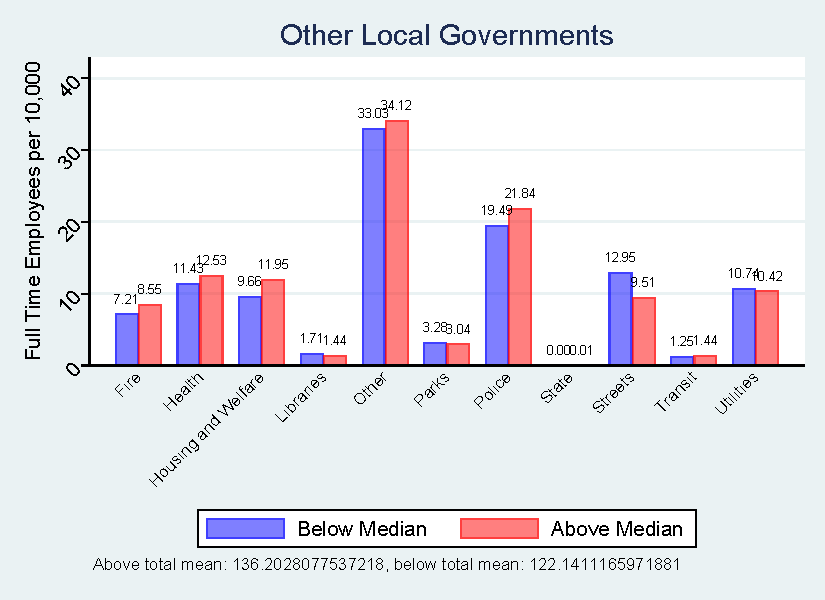
\includegraphics{figures/implications/spdist_emp_ft_0.pdf}
\end{figure}
\begin{figure}
	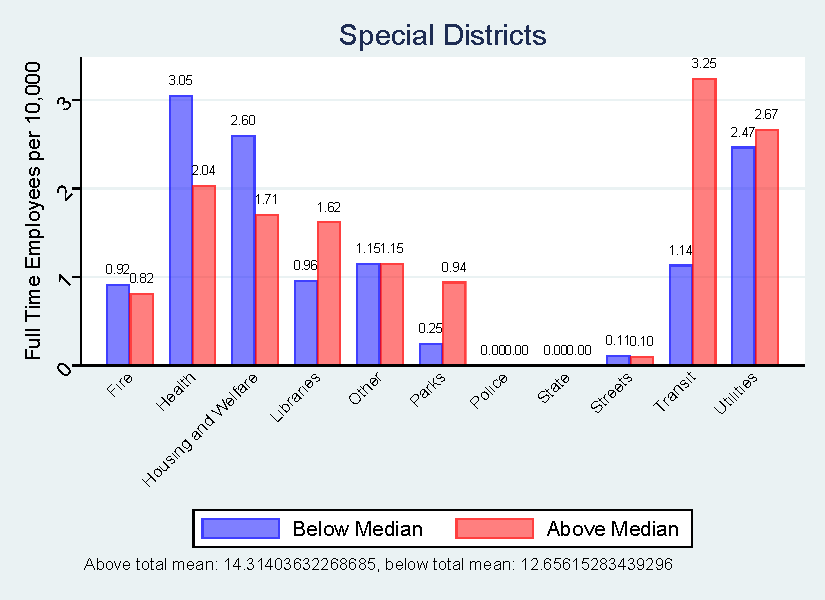
\includegraphics{figures/implications/spdist_emp_ft_1.pdf}
\end{figure}
\clearpage
\begin{figure}
	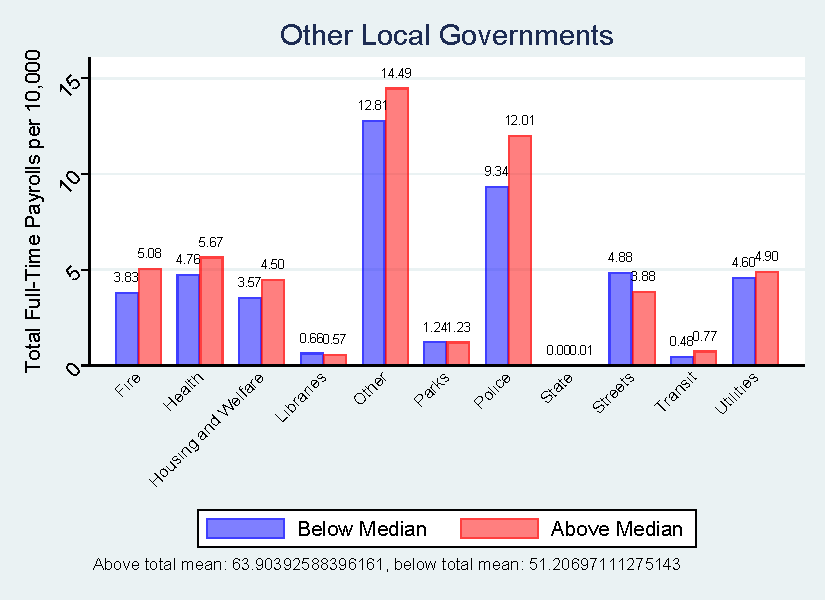
\includegraphics{figures/implications/spdist_emp_p_ftp__0.pdf}
\end{figure}
\begin{figure}
	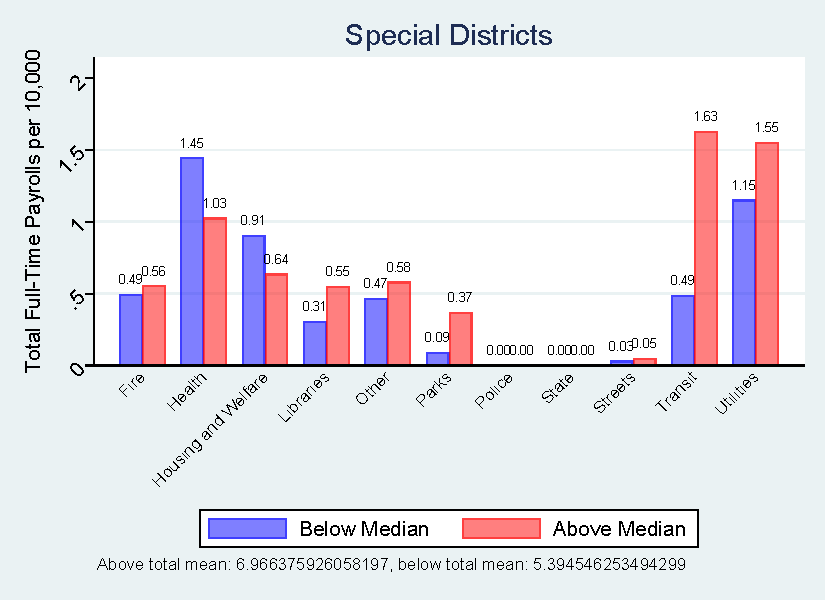
\includegraphics{figures/implications/spdist_emp_p_ftp__1.pdf}
\end{figure}
\clearpage
\begin{figure}
	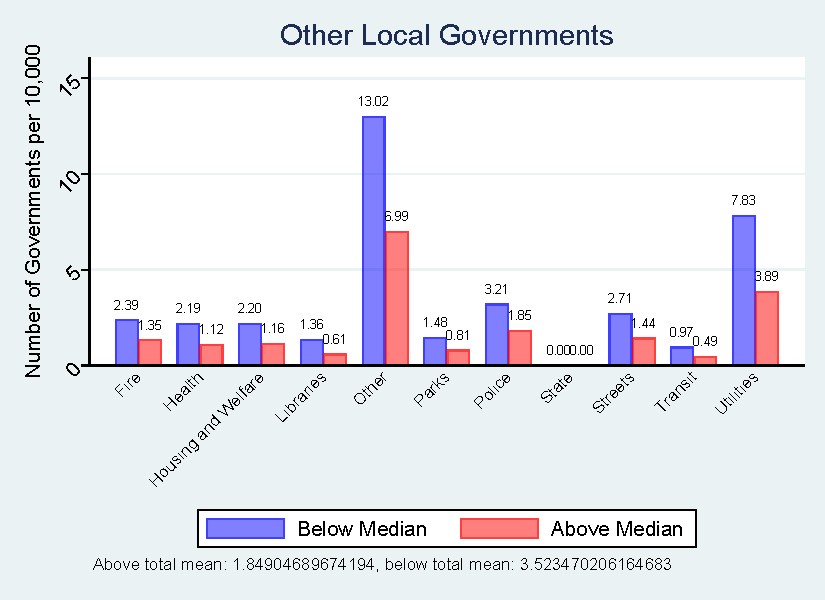
\includegraphics{figures/implications/spdist_emp_pc_0.pdf}
\end{figure}
\begin{figure}
	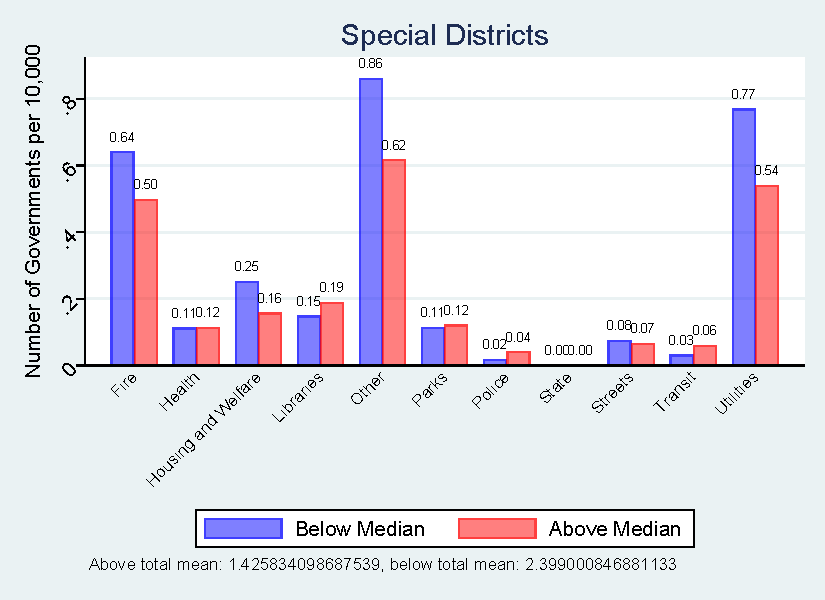
\includegraphics{figures/implications/spdist_emp_pc_1.pdf}
\end{figure}
\clearpage
\begin{figure}
	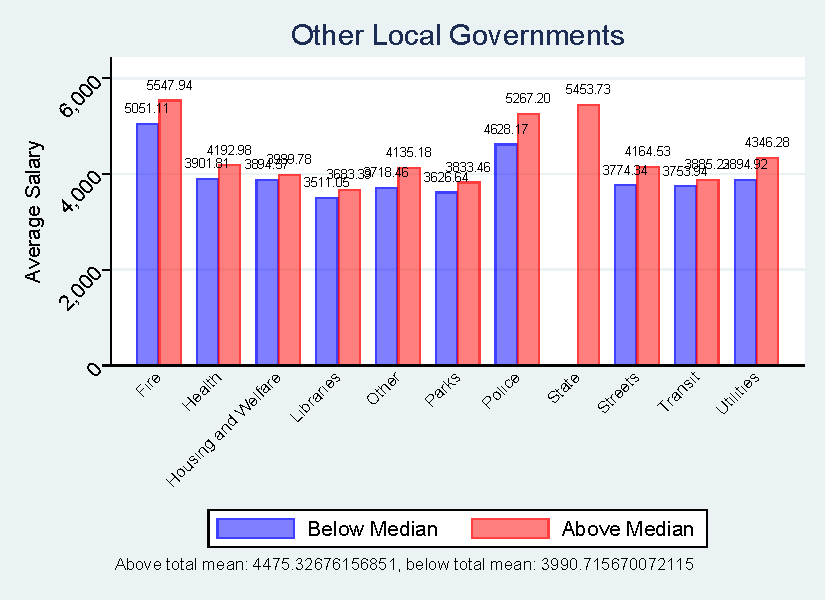
\includegraphics{figures/implications/spdist_emp_salary__0.pdf}
\end{figure}
\begin{figure}
	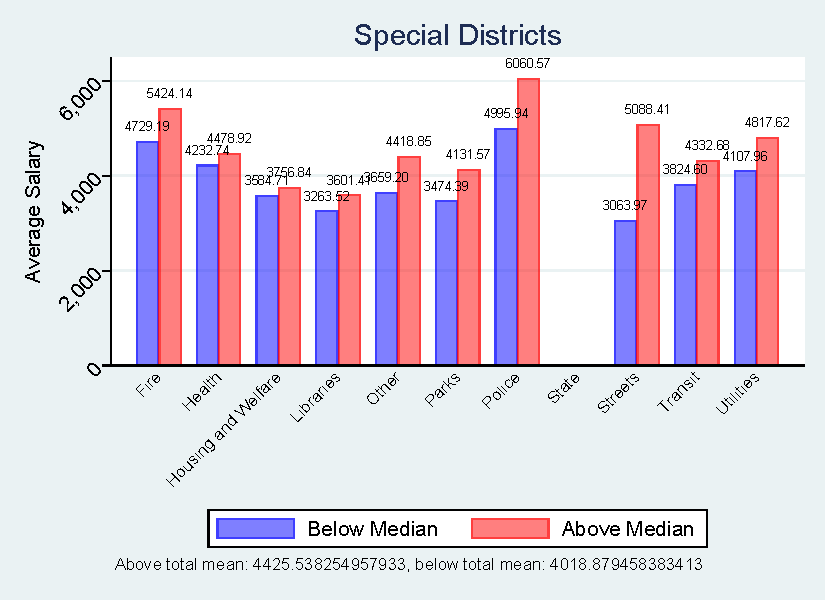
\includegraphics{figures/implications/spdist_emp_salary__1.pdf}
\end{figure}
\clearpage
\end{document}